\section{色彩迁移实验}

\subsection{色彩迁移方法}
\begin{frame}{当前章节}
    \tableofcontents[currentsection, currentsubsection]
\end{frame}

\begin{frame}{色彩迁移方法} 
    \begin{description}
        \item[HM] histogram matching 经典直方图匹配方法
        \item[reinhard] color transfer between images, 2001, 在正交的$I, \alpha, \beta$空间中变换
        \item[MKL] Monge-Kantorovich Linearization, 2007, 最优传输的思想引入色彩迁移
        \item[MVGD] Multi-Variate Gaussian Distributions, 在色彩迁移中引入多元高斯分布, 2007
    \end{description}
    
\end{frame}

\subsection{色彩迁移实验结果}
\begin{frame}{当前章节}
    \tableofcontents[currentsection, currentsubsection]
\end{frame}

\begin{frame}{色彩迁移实验结果}
    \begin{figure}[!htbp]
        \centering
        \subfloat[{\tiny hm: ssim 0.3807 - 0.3860; pnsr 16.59 - 17.43}]{\label{fig:0201a}
        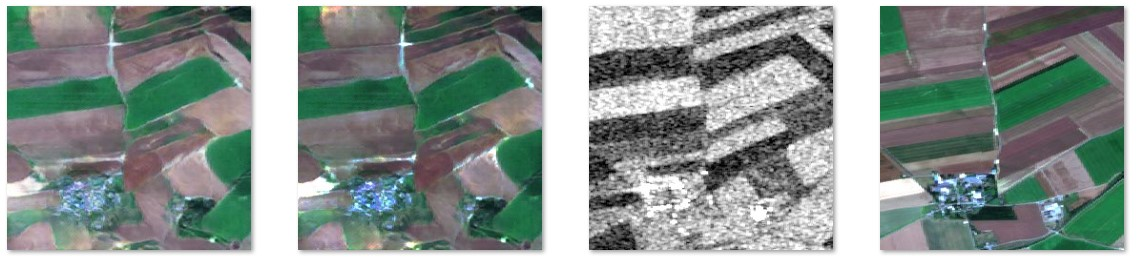
\includegraphics[height=1.5cm]{pic/chap02hm02.jpg}}
        \\[0.1cm]
        \subfloat[{\tiny mkl: ssim 0.3465 - 0.3484; pnsr 14.19 - 14.30}]{\label{fig:0201b}
        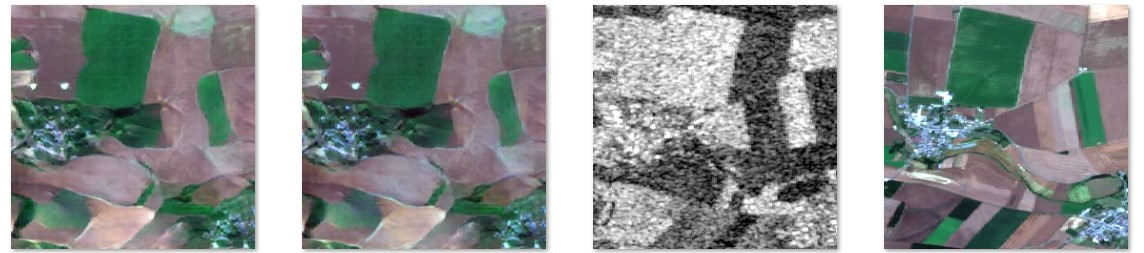
\includegraphics[height=1.5cm]{pic/chap02mkl03.jpg}}
        \\[0.1cm]
        \subfloat[{\tiny rh: ssim 0.2549 - 0.2707; pnsr 11.22 - 11.59}]{\label{fig:0201c}
        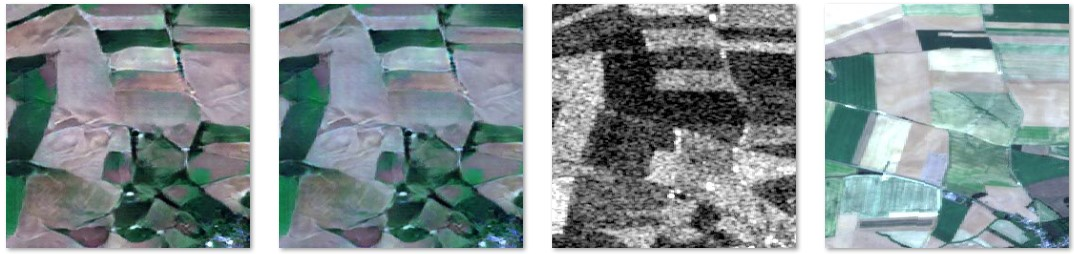
\includegraphics[height=1.5cm]{pic/chap02reinhard01.jpg}}
        \label{fig:0201}
    \end{figure}
\end{frame}

\subsection{工作计划}
\begin{frame}{当前章节}
    \tableofcontents[currentsection, currentsubsection]
\end{frame}

\begin{frame}{工作计划}
    对于metaSR任意比例超分实验
    \begin{itemize}
        \item 高版本代码配置环境训练metaSR
        \item 用自己的数据重新训练而非下采样
    \end{itemize}

    对于图像翻译实验:
    \begin{itemize}
        \item 重新整理pix2pix数据集, 进行训练
    \end{itemize}
\end{frame}

